% CVPR 2022 Paper Template
% based on the CVPR template provided by Ming-Ming Cheng (https://github.com/MCG-NKU/CVPR_Template)
% modified and extended by Stefan Roth (stefan.roth@NOSPAMtu-darmstadt.de)

\documentclass[10pt,twocolumn,letterpaper]{article}

%%%%%%%%% PAPER TYPE  - PLEASE UPDATE FOR FINAL VERSION
%\usepackage[review]{cvpr}      % To produce the REVIEW version
\usepackage{cvpr}              % To produce the CAMERA-READY version
%\usepackage[pagenumbers]{cvpr} % To force page numbers, e.g. for an arXiv version

% Include other packages here, before hyperref.
\usepackage{graphicx}
\usepackage{amsmath}
\usepackage{amssymb}
\usepackage{booktabs}


% It is strongly recommended to use hyperref, especially for the review version.
% hyperref with option pagebackref eases the reviewers' job.
% Please disable hyperref *only* if you encounter grave issues, e.g. with the
% file validation for the camera-ready version.
%
% If you comment hyperref and then uncomment it, you should delete
% ReviewTempalte.aux before re-running LaTeX.
% (Or just hit 'q' on the first LaTeX run, let it finish, and you
%  should be clear).
\usepackage[pagebackref,breaklinks,colorlinks]{hyperref}


% Support for easy cross-referencing
\usepackage[capitalize]{cleveref}
\crefname{section}{Sec.}{Secs.}
\Crefname{section}{Section}{Sections}
\Crefname{table}{Table}{Tables}
\crefname{table}{Tab.}{Tabs.}


%%%%%%%%% PAPER ID  - PLEASE UPDATE
\def\cvprPaperID{*****} % *** Enter the CVPR Paper ID here
\def\confName{CVPR}
\def\confYear{2023}


\begin{document}

%%%%%%%%% TITLE - PLEASE UPDATE
\title{Project Progress Report: \\Aug-NeLF: Augmented Neural Light Fields with Stronger Multi-View Consistency}

\author{Zhiyuan Ren, Han Meng, Maolin Gan, Lanpeng Li\\
Michigan State University\\
428 S Shaw Ln 3115, East Lansing, MI 48824\\
{\tt\small renzhiy1@msu.edu, menghan1@msu.edu, ganmaoli@msu.edu, lilanpen@msu.edu}
% For a paper whose authors are all at the same institution,
% omit the following lines up until the closing ``}''.
% Additional authors and addresses can be added with ``\and'',
% just like the second author.
% To save space, use either the email address or home page, not both
% \and
% Second Author\\
% Institution2\\
% First line of institution2 address\\
% {\tt\small secondauthor@i2.org}
}
\maketitle

%%%%%%%%% ABSTRACT
\begin{abstract}
   Compared with Neural Radiance Field(NeRF), Neural Light Field(NeLF) can render 2D images with novel views from neural representation of 3D scenes without multiple sampling along the ray, which makes real-time rendering possible. One shortcoming of the NeLF is lack of the multi-view consistency or geometric structure due to the sparse feature representation space. Recently, robust data augmentation have reached great success for improving the generalization and robustness of the model. Inspired by this, we hope robust data augmentation can bring its power to NeLF by learning from perturbed data, thus improving the multi-view consistency. For the next 45 days, we plan to establish the baseline setting within two weeks and then tune the basic methods as we get more inspiring experimental results within three weeks. Last we use around a week to finish the writing job.
\end{abstract}

%  
%%%%%%%%% BODY TEXT
\section{Introduction}
\label{sec:intro}
Inverse rendering from 3D scene is a fundamental problem both in computer vision and computer graphics. Recent research in modeling implicit neural representations \cite{dellaert2020neural, mescheder2019occupancy, park2019deepsdf, takikawa2021neural} and rendering in the differential way \cite{mildenhall2021nerf} has advanced the progress of this problem. Especially, Neural Radiance Field(NeRF) and its variants have reached great success due to the straightforward optimization by the MLP and differential volumetric rendering. However, the inference of NeRF needs to sample many points along each ray and feed these points into the neural network one by one, which make it difficult to do real-time rendering.

\begin{figure*}
  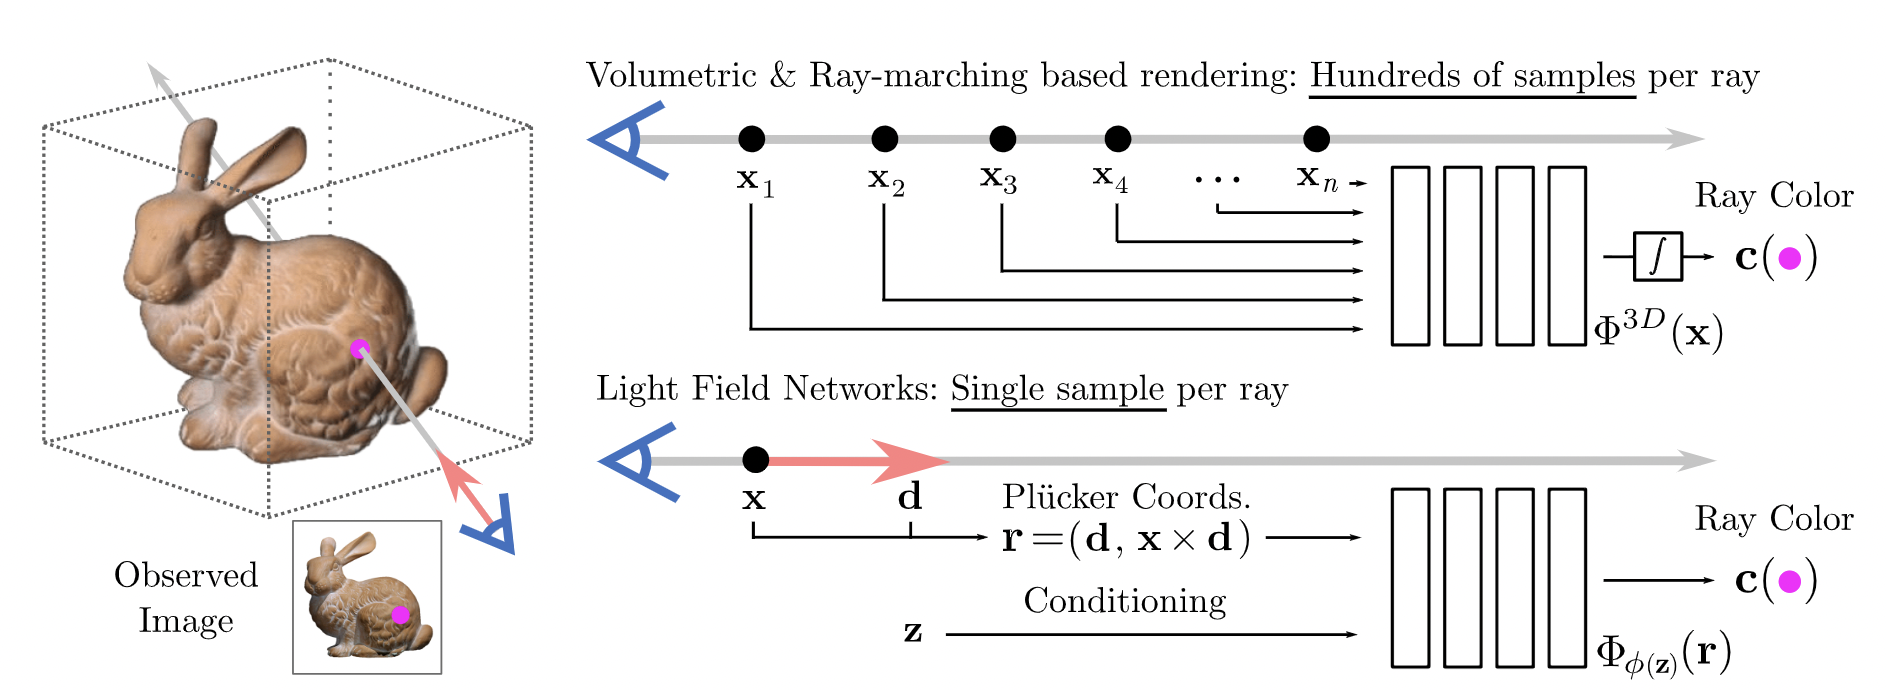
\includegraphics[width=\textwidth,height=6cm]{figures/nerf_vs_nelf.png}
  \caption{Comparison between Neural Radiance Field(NeRF) and Neural Light Field(NeLF).}
  \label{fig1}
\end{figure*}

To tackle this problem, people proposed Neural Light Field(NeLF) \cite{sitzmann2021light} which directly map a ray passing through one pixel to the radiance value. Different from NeRF(shown in Fig.\ref{fig1}), NeLF does not need to query opacity at 3D locations along a ray and regress the color value with the four dimensional space of light rays, which speed up rendering process a lot. As every coin has two sides, NeLF suffers from bad multi-view consistency because it does not model the density explicitly as NeRF, leading to sparse feature representation space and difficult optimization. There has been several works studying to solve this problem. \cite{sitzmann2021light} uses meta learning to learn a strong prior to improve the geometry consistency. \cite{attal2022learning} projects the low dimensional input into higher dimensional embedding to feed richer representation into neural network. \cite{wang2022r2l} adopts distillation to help NeLF learn the multi-view consistency and geometry information from well pre-trained NeRF. 

Inspired by recent work Aug-NeRF \cite{chen2022aug}, which applies robust data augmentation strategy to NeRF and helps improve inconsistent and visually non-smooth geometric results, we think that NeLF lacks more multi-view consistency and geometry information and naturally we propose Aug-NeLF. Training procedure will injects different level perturbations including input coordinates, feature level representation and output color. Hopefully, our Aug-NeLF can efficiently solve the multi-view inconsistency problem in Neural Light Field area. Our codes are available in \url{https://github.com/Zhiyuan-VisionKing/Aug-NeLF}
%------------------------------------------------------------------------
\section{Related Work}
\label{sec:formatting}
\textbf{Aug-NeRF}. Aug-NeRF addresses the inherent non-smooth geometries of NeRF. Specifically, based on solid physical grounds, Aug-NeRF seamlessly injects worst-case perturbations into three levels of the NeRF pipeline, leading to substantially improved geometry continuity and generalization ability. Moreover, the implicit smooth prior induced by triple-level augmentation enables NeRF to recover scenes from noisy supervision images. Considering that Aug-NeRF has reached great success and NeLF need more geometry consistency than NeRF, we judge that it is feasible to improve the performance of the NeLF model.

%------------------------------------------------------------------------
\section{Method}
Designing dedicated perturbations for NeLF is far from trivial due to its inherent physics. We propose to inject worst-case perturbations into all three levels:  coordinates,intermediate features of MLP, and pre-rendering MLP output:all with clear physical meanings.  Formally, our approach
$$
\min _{\Theta} \mathbb{E}_{(\boldsymbol{r}, \widehat{\boldsymbol{C}}) \sim \mathbb{P}(\mathcal{R})}^{\max _{\boldsymbol{\delta}}}\left\|\boldsymbol{C}^{\dagger}(\boldsymbol{r} \mid \Theta, \boldsymbol{\delta})-\widehat{\boldsymbol{C}}\right\|_2^2,
$$
where $\boldsymbol{\delta}=\left(\boldsymbol{\delta}_p, \boldsymbol{\delta}_f, \boldsymbol{\delta}_r\right) \in \mathcal{S}_p \times \mathcal{S}_f \times \mathcal{S}_r$
where $\delta_p, \delta_f$, and $\delta_o$ are the perturbations to be learned and injected to the input coordinate, intermediate MLP feature, and pre-rendering RGB- $\sigma$ output, respectively, where $\mathcal{S}_p \subseteq \mathbb{R}^6, \mathcal{S}_f \subseteq \mathbb{R}^D$, and $\mathcal{S}_r \subseteq \mathbb{R}^4$ are the corresponding perturbation search range, $D$ is the hidden dimension of the MLP. We elaborate on each perturbation as below.

The perturbations can be accurately estimated by multi-step Projected Gradient Descent (PGD). Taking $\ell_{\infty}$ norm ball for example:
$$
\boldsymbol{\delta}^{(t+1)}=\prod_{\|\boldsymbol{\delta}\|_{\infty} \leq \epsilon}\left[\boldsymbol{\delta}^{(t)}+\alpha \cdot \operatorname{sgn}\left(\nabla_{\boldsymbol{\delta}} \mathcal{L}(\Theta \mid \mathcal{R}, \boldsymbol{\delta})\right]\right.
$$
where $\alpha$ is the step size of the inner maximization, $\Pi[\cdot]$ denotes a projection operator, $\operatorname{sgn}(\cdot)$ takes the sign of the input, and $\mathcal{L}(\Theta \mid \mathcal{R}, \boldsymbol{\delta})$ represents the MSE loss between perturbed color $\boldsymbol{C}^{\dagger}$ and ground-truth color $\widehat{C}$.
%------------------------------------------------------------------------
\section{Experiments}
\label{sec:formatting}
\textbf{NeLF}.
%%%%%%%%% REFERENCES
{\small
\bibliographystyle{ieee_fullname}
\bibliography{egbib}
}

\end{document}
